\section{Caracterización de columnas atómicas}

Una vez conocemos la posición de cada columna atómica, necesitamos generar y asignarles una firma que nos permita clasificar las distintas especies de columnas en función del tipo de átomo que representan. Dichas firmas, mejor conocidas como vectores de características (\textit{feature vectors}), serán el input que suministremos a una red neuronal y/o algoritmos de \textit{clustering} para clasificar las distintas columnas atómicas presentes en cierta imagen ADF.\\

En nuestro caso, la información necesaria para caracterizar a cada columna la extraemos fijándonos en cómo se posicionan sus vecinos más próximos. Para cada átomo tomamos de la imagen original un pequeño parche $m \times m$ (ver \autoref{fig:8}) y lo almacenamos en un tensor $m \times m \times n$, donde n corresponderá con el número total de parches. Posteriormente, aplanamos cada sección $m \times m$ para generar vectores de longitud $m^2$, de modo que finalmente nos quedaremos con una matriz $X$ de dimensiones $n \times m^2$. En las siguientes secciones trataremos de procesar toda esta información para generar la firma de cada una de nuestras columnas atómicas.

\begin{figure}[h!]
    \centering
    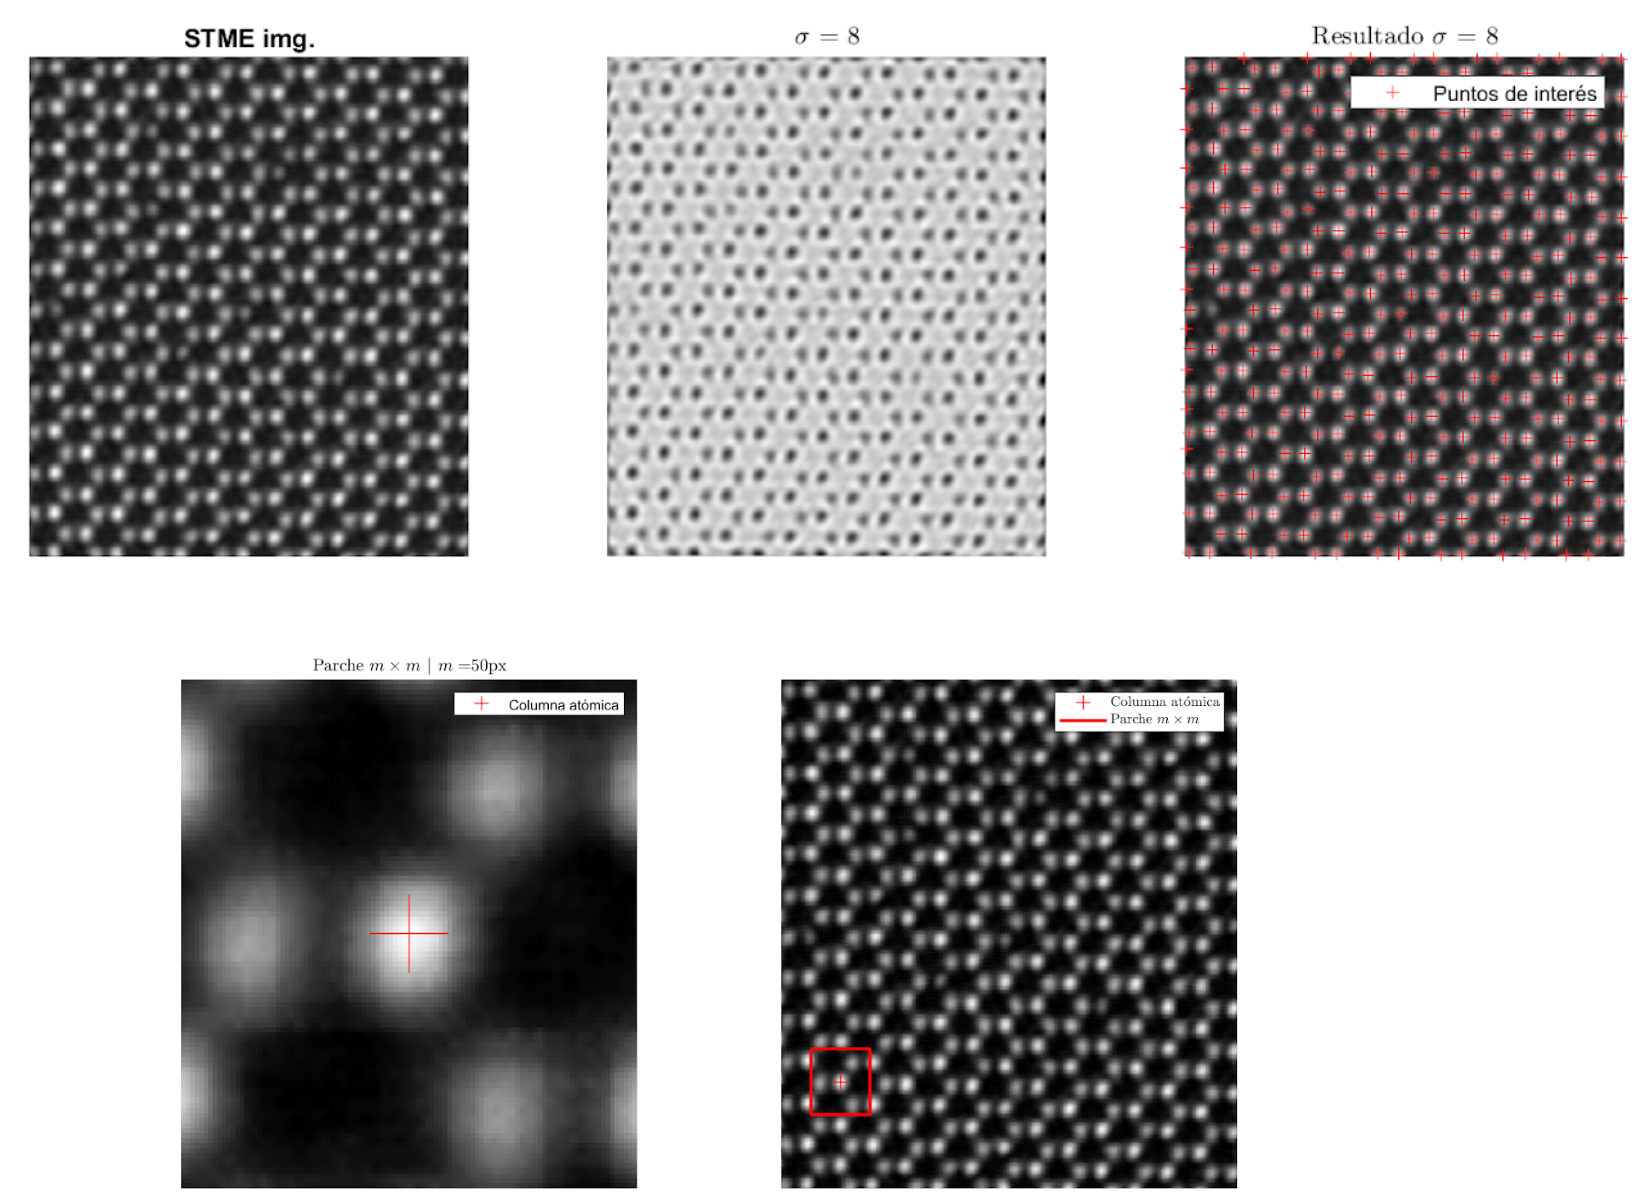
\includegraphics[width=0.8\textwidth]{fig/Fig8.png}
    \caption{Para imagen ADF de MoSe$_2$, adaptada de la referencia \cite{ml}, se muestra el resultado del algoritmo de detección de columnas atómicas y la escala de los parches que se han seleccionado para caracterizarlas. Programa desarrollado en MATLAB por el autor \cite{repo}.}
    \label{fig:8}
\end{figure}

\newpage
\subsection{Métodos de factorización matricial}

Al estar codificando nuestros datos en forma matricial, podemos plantear la caracterización de las columnas como un problema de reducción de dimensionalidad. Trataremos a las n filas como distintas observaciones y a las $m^2$ columnas como las distintas variables que se pueden medir en cada observación.\\

La idea será descomponer la matriz $X$ en las matrices $V$ ($p \times m^2$) y $U$ ($n \times p$), de modo que $X = U \times V$. La dimensión p coincidirá con el número de componentes que contendrá el vector de características de cada columna atómica. Estos métodos se aplican principalmente en reducción de dimensionalidad porque típicamente $p \ll m^2$.

\begin{figure}[h!]
    \centering
    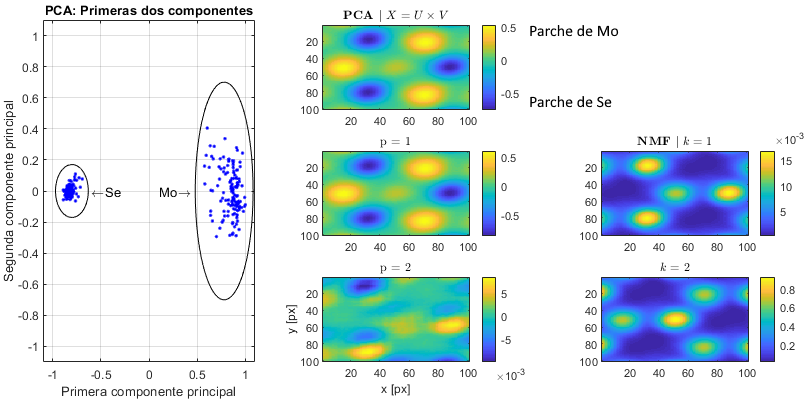
\includegraphics[width=1\textwidth]{fig/Fig9.png}
    \caption{Para la misma imagen ADF de MoSe$_2$ que aparece en la \autoref{fig:8}, se muestran los resultados tras aplicar PCA, quedándonos con únicamente las dos primeras componentes, y NMF para un máximo de $k = 2$. Programa desarrollado en MATLAB por el autor \cite{repo}, reproduce los resultados expuestos en \cite{ml}.}
    \label{fig:9}
\end{figure}

\vspace{-0.5cm}
\subsubsection{\textit{Principal component analysis} (PCA)}
El PCA es una técnica que, haciendo uso de la descomposición SVD, nos ofrece un sistema de coordenadas que toma como base las direcciones de máxima variación. Esto resulta muy útil para \textit{datasets} que cuentan con una gran correlación entre algunas de sus entradas, pues seremos capaces de reducir drásticamente la cantidad de variables necesarias para distinguir entre sus distintas clases de observaciones. Para computar este algoritmo inicialmente se genera la matriz $B$ substrayendo la media de la filas de $X$:

\begin{equation}
    B = X - \bar X \quad \text{donde} \quad
    \bar X = 
    \begin{bmatrix}
    1        \\
    \vdots   \\
    1        \\
    \end{bmatrix} \bar x \quad \text{y} \quad
    \bar x_j = \frac{1}{n} \sum^n_{i=1} X_{ij}.
\end{equation}

\begin{wrapfigure}{o}{9cm}
    \centering
    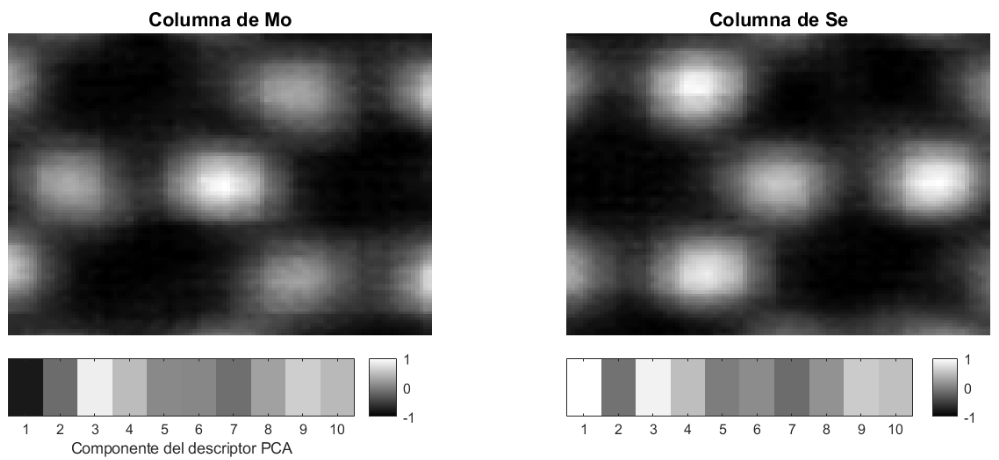
\includegraphics[width=0.5\textwidth]{fig/Fig10.png}
    \caption{En función de los resultados obtenidos en la \autoref{fig:9} con PCA, se toman dos columnas atómicas arbitrarias (una de Mo y otra de Se) y se determinan sus vectores descriptores resultantes tras seleccionar $p = 10$ componentes principales. Programa desarrollado en MATLAB por el autor \cite{repo}.}
    \label{fig:10}
\end{wrapfigure} 

Una vez tenemos $B$, ya todo se reduce a aplicar el método SVD. Los autovectores asociados a los valores singulares más grandes corresponderán con las direcciones de mayor variación.\\



En las Figuras \ref{fig:9} y \ref{fig:10} se muestran algunos de los resultados obtenidos por PCA. Observamos que, aunque logramos separar perfectamente los dos tipos de átomos, al contar con coordenadas negativas, es complicado encontrar una conexión entre las componentes principales y la física de las columnas atómicas


\subsubsection{\textit{Non-negative matrix factorization} (NMF)}

La NMF soluciona el problema de interpretabilidad del PCA, aportando una representación sin coordenadas negativas que respeta las restricciones físicas. Este hecho permite a la NMF realizar \textbf{mapas de fases} sobre imágenes ADF, como los que se ven en la \autoref{fig:11}.\\

En el caso de la \autoref{fig:9} se realiza una NMF para dos componentes, lo que nos aporta una imagen promedio para cada tipo de parche.

\begin{figure}[h!]
    \centering
    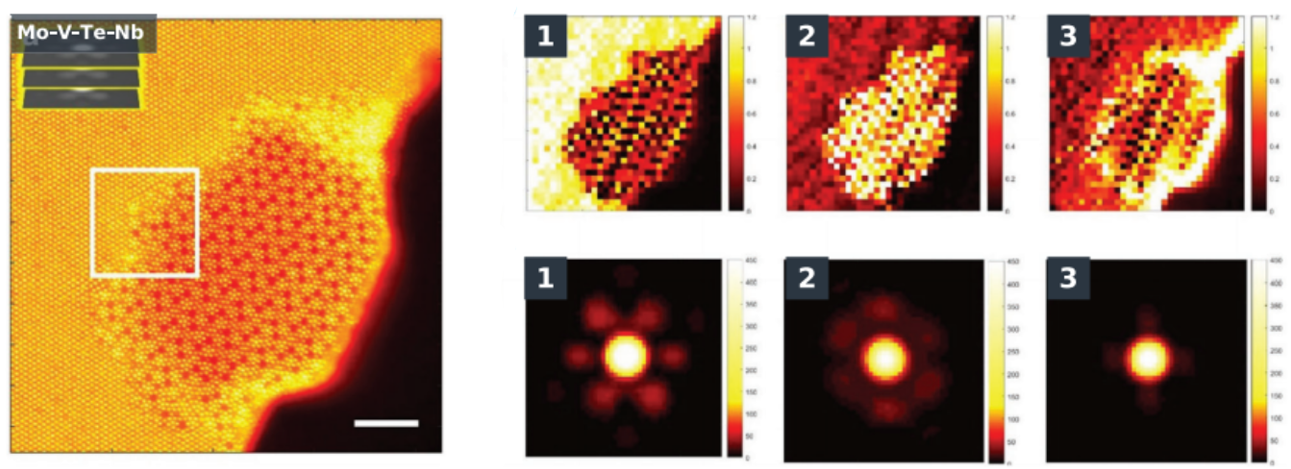
\includegraphics[width=1\textwidth]{fig/Fig11.png}
    \caption{Figura adaptada de la referencia \cite{ml}. Tenemos una imagen ADF de Mo-V-Te-Nb sobre la que se ha aplicado NMF de tres componentes. De seguido encontramos los mapas de fase ($X = U \times V$) y su autovector asociado (reescalado de de las filas de $V$).}
    \label{fig:11}
\end{figure}
